\section{Ausgangslage}
Die Agentur allink.creative ist im letzten Jahr stark gewachsen. Von zehn
Mitarbeitern im Februar 2010 auf siebzehn Mitarbeiter im Februar 2011. Dies hat 
zur Auswirkung, dass gewisse Abläufe und Prozesse neu definiert und bestehende
überarbeitet werden müssen, um weiterhin effizient, oder wenn möglich noch 
effizienter, arbeiten zu können. Die Agentur arbeitet zurzeit überwiegend mit Apple
Computern und setzt gewisse Software ein, die die Geschäftsleitung beibehalten 
möchte. Es soll jedoch innerhalb dieser Arbeit geprüft werden, welche Software
weiterhin Sinn macht und welche man möglicherweise ersetzen oder neu anschaffen
bzw. sogar selbst entwickeln möchte.

\section{Problemstellung}
Durch den schnellen Wachstum der Agentur stösst sie bei der Abwicklung ihrer
Projekte an Grenzen. Die Partner, die bisher den Überblick über alle
Projekte und deren Abläufe im Auge behalten konnten, sind bei dieser Grösse
nicht mehr in der Lage dies beizubehalten. Deshalb muss mehr Struktur geschaffen und
den Mitarbeitern mehr Verantwortung und Kompetenzen abgegeben werden. Und trotzdem
soll es der Geschäftsleitung mit Hilfe von Controling Tools möglich bleiben,
einen Überblick über die Lage der Agentur zu behalten.

Die Partner erhoffen sich dadurch ein gesundes Wachstum der Agentur ermöglichen
zu können. Zusätzlich wird vermutet, dass durch Optimierungen im Projektablauf
auch Kosten gespart werden können und die ganze Agentur im Allgemeinen 
professionalisiert werden kann.

\section{Zielsetzung}
Das Hauptziel dieser Arbeit besteht darin, das aktuelle Projektmanagement der 
allink zu analysieren, den zur Zeit gegebenen Umständen anzupassen und zu
optimieren, damit ein weiteres Wachstum der Agentur vereinfacht wird.

Allen Partnern bei der allink ist klar, dass der heutiger Projektablauf 
nicht optimal ist. Zu oft sehen sie sich mit gleichen Problemen konfrontiert, 
die in anderen Projekt schon einmal angetroffen und gelöst wurden.
Jedes Mal wird versucht daraus zu lernen, ohne etwas konkret festzuhalten oder
wirklich zu verändern. Das liegt meist daran, dass zu viel ansteht und
die internen Verbesserungen hinter die Aufträge und Wünsche der Kunden
gestellt werden.

Der aktuellen Projektablauf der allink wird genauer untersucht und auf 
dessen Stärken und Schwächen eingegangen. Danach werden die Bedürfnisse und 
Anforderungen der verschiedenen Stakeholdern des Projektablaufes aufgenommen und
Kennzahlen definiert, die in Zukunft bei einem verbesserten Projektablauf gemessen 
werden sollen. Daraus wird ein neues Konzept des überarbeiteten Projektablaufes 
mit verschiedenen Varianten in der Umsetzung erstellt und zusammen mit der 
Geschäftsleitung der allink entschieden, welchen Projektablauf 
man in Zukunft einsetzen und verfeinern möchte. Der neue Projektablauf soll 
abschliessend in einem ``Proof of Concept'', also anhand eines konkreten Projektes, 
getestet werden.

\section{Aufbau der Arbeit}
Im Kapitel \ref{chap:theorie_teil} werden dem Leser die Grundlagen zu Projektmanagement 
näher gebracht. Neben den jeweiligen Begriffserklärungen werden wichtige Modelle 
und Tools aus der Theorie und Praxis aufgezeigt.

Im Kapitel \ref{chap:analyse} wird der aktuelle Projektablauf bei der allink
GmbH genauer analysiert und aufgezeigt. Mit Hilfe der Prozessdarstellung wird
das aktuelle Vorgehen dargestellt und mit Beispielen untermalt. In einem
Branchenvergleich werden ähnlich grosse Agentur interviewt und deren Vorgehen
als Vergleich herangezogen.

Im Kapitel \ref{chap:anforderungen} werden die Bedürfnisse und Anforderungen 
aller Stakeholders die in den Projektablauf involviert sind aufgenommen und daraus
Anforderungen gebildet. Zusätzlich werden Kennzahlen definiert, die in Zukunft
während und nach den Projekten gemessen werden sollen.

Im Kapitel \ref{chap:konzept} wird ein Konzept des neuen Projektablaufes
erarbeitet und verschieden Varianten zur Umsetzung aufgezeigt. Auf dieser Grundlage
entscheidet sich der Auftraggeber für einen neuen Projektablauf. Dieser wird
im Kapitel \ref{chap:proof_of_concept} der Arbeit in einem ``Proof of Concept'' 
getestet.

Im letzten Kapitel \ref{chap:reflektion} wird die Arbeit in Form eines Fazits 
zusammengefasst. Zudem wird ein Ausblick auf die zukünftige Verwendung und den 
Einsatz des neuen Projektablaufes abgegeben.

Die folgende Abbildung \ref{pic:01_gliederung_arbeit} beschreibt die Gliederung der 
Arbeit in graphischer Form und zeigt auf, wie die erarbeiteten Resultate in
das Konzept des neuen Projektablaufes einfliessen.

\begin{figure}[htbp]
\begin{center}
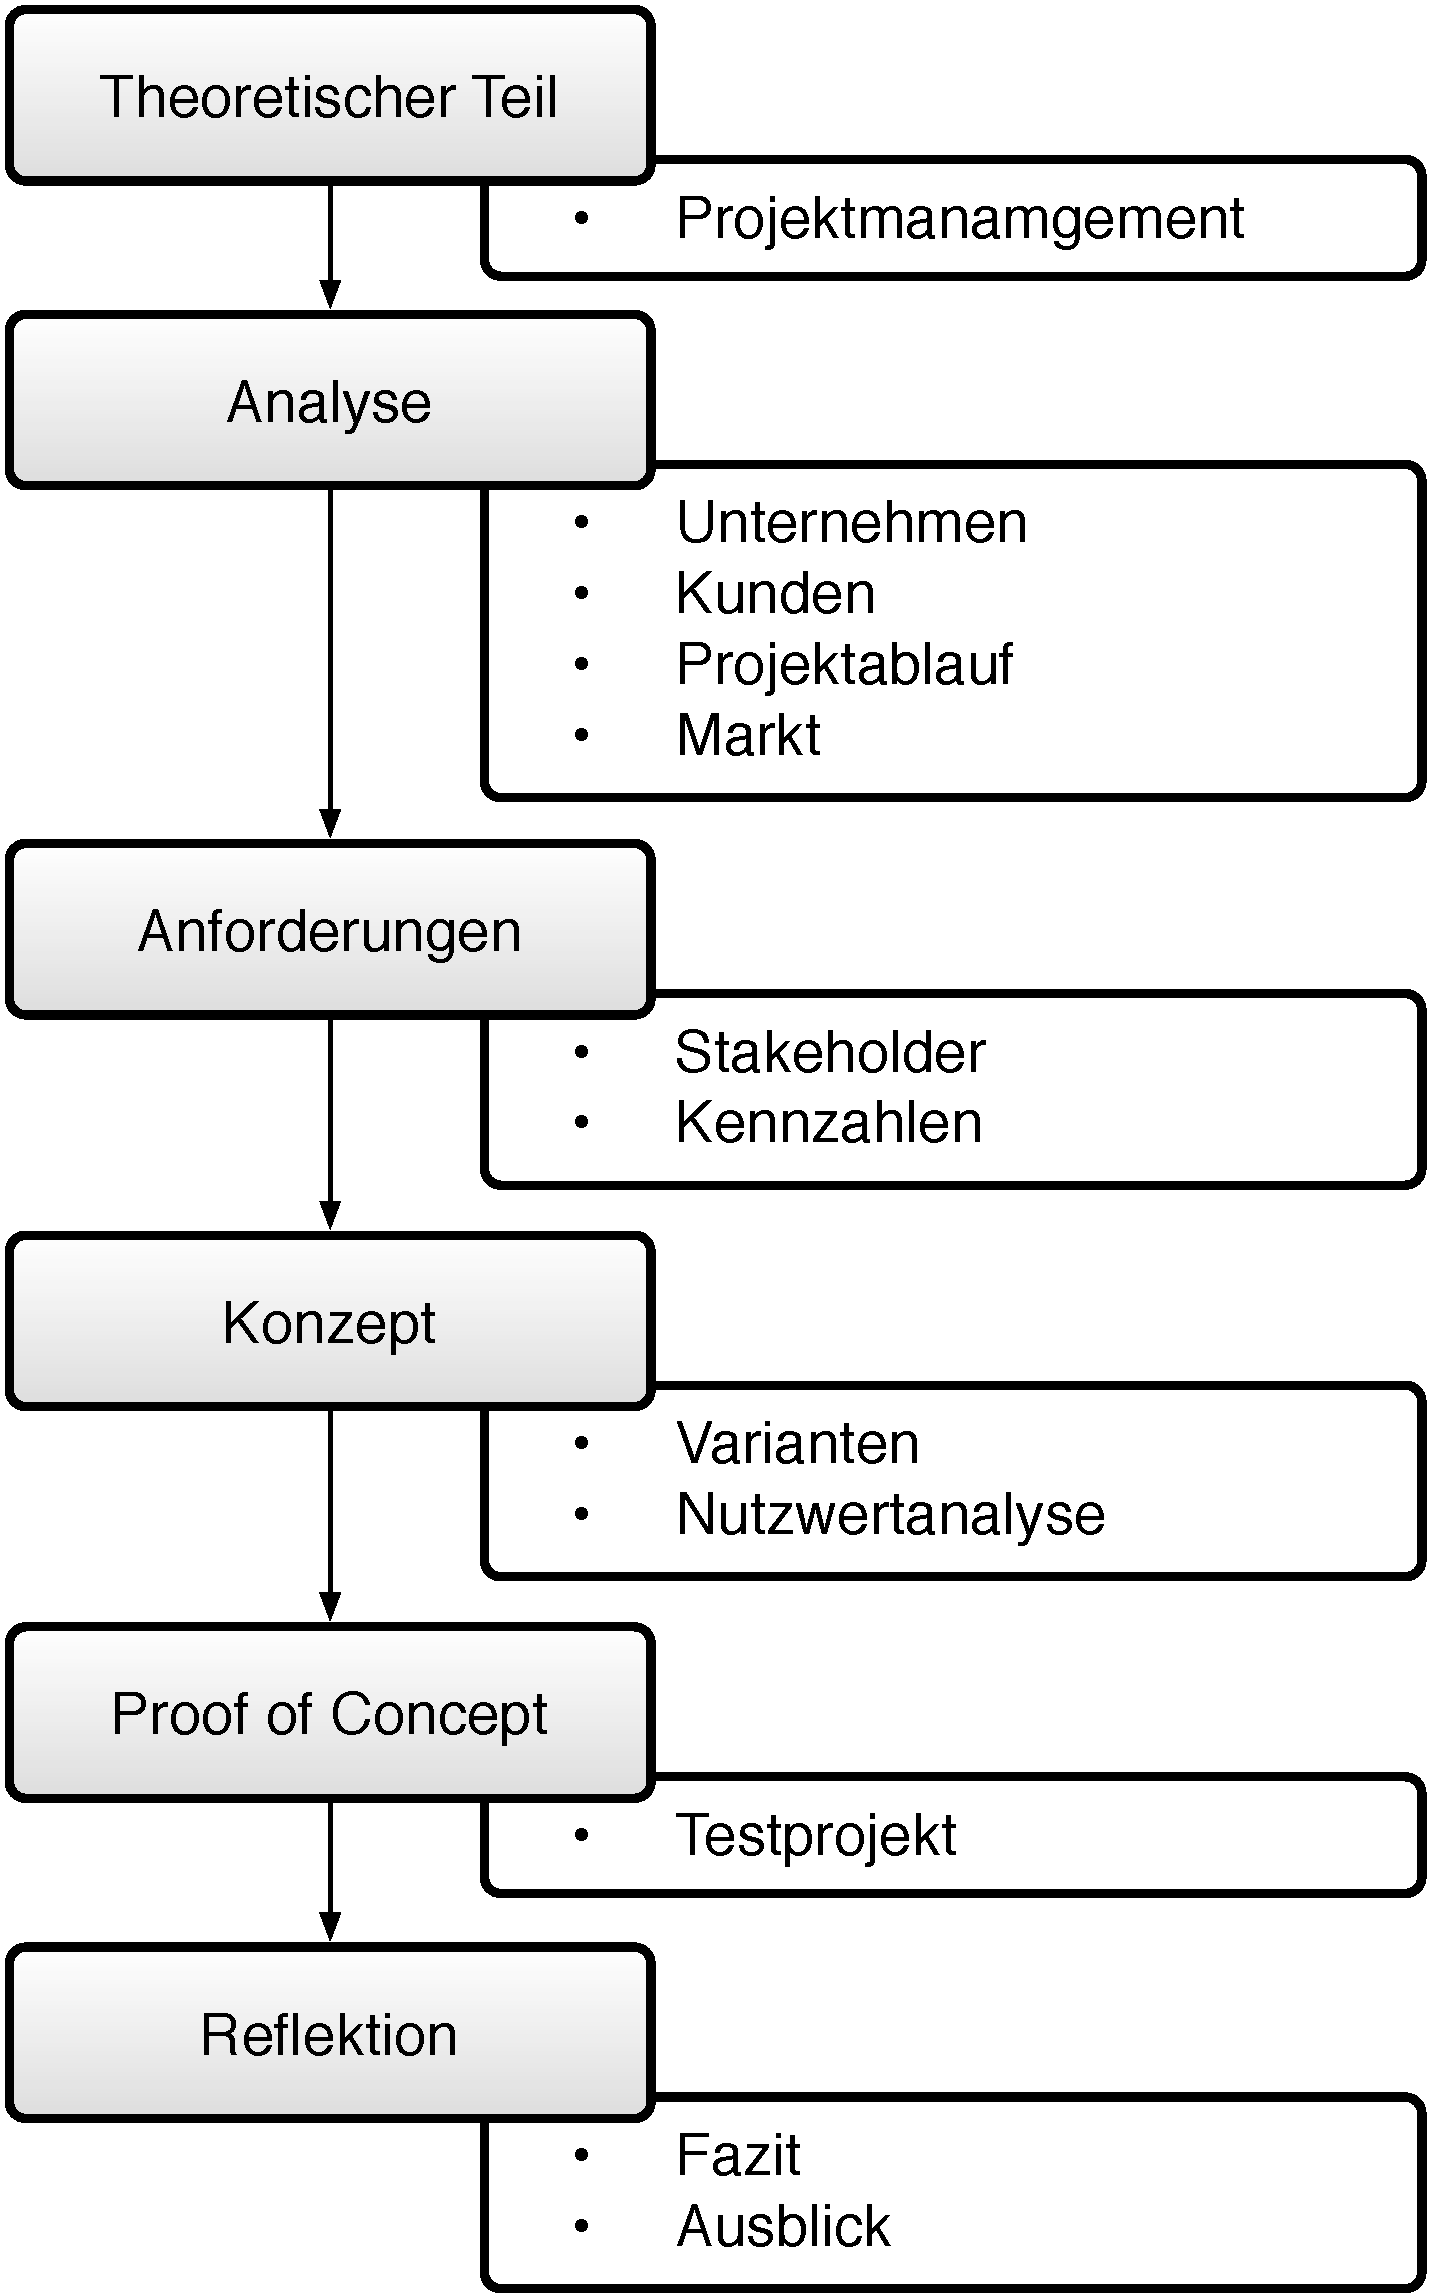
\includegraphics[width=0.6\textwidth,angle=0]{./bilder/einleitung/01_gliederung_arbeit.pdf}
\caption[Aufbau der Diplomarbeit]{Aufbau der Diplomarbeit\footnotemark}
\label{pic:01_gliederung_arbeit}
\end{center}
\end{figure}
\footnotetext{Eigene Darstellung}

\section{Inhaltliche Schwerpunkte}
Die inhaltlichen Schwerpunkte dieser Arbeit liegen in den folgenden Bereichen:

\begin{itemize}
    \item Einarbeitung Theorie Projektmanagement
    \item Analyse des aktuellen Projektablaufes der allink GmbH
    \begin{itemize}
        \item Darstellung des Projektablaufes
        \item Aufzeigen der Stärken und Schwächen
        \item Zurzeit verwendete Software und Hilfsmittel
    \end{itemize}
    \item Aufnahme der Bedürfnisse und Anforderungen an den Projektablauf
    \item Konzept eines neuen Projektablaufes
    \begin{itemize}
        \item Erarbeitung von praxisnahen Varianten
        \item Aufzeigen von unterstützender Software und Hilfsmittel
    \end{itemize}
    \item ``Proof of Concept'' des Projektablaufes mit den gewählten Varianten
    \item Fazit und Reflektion der Arbeit
\end{itemize}

Die Arbeit soll dem Leser und anderen Agenturen in einer ähnlichen Situation
aufzeigen, was für Herausforderungen bei einem Wachstum entstehen und wie
sie mit Hilfe von Veränderungen und Anpassungen bewältigt werden können.

\section{Inhaltliche Ein- und Abgrenzung}
Die Arbeit fokussiert sich auf eine Agentur. Es wird vertieft auf deren Probleme
und Herausforderungen eingegangen. Deshalb sind die Schlüsse die darin gezogen
werden nicht grundsätzlich für jede Agentur anwendbar. Es wird jedoch versucht, das
ganze so global wie möglich zu betrachten. Da zum Schluss aber eine für die
Agentur in der Praxis anwendbare neue Lösung gesucht wird, passt diese wohl
kaum in jede Firmenkultur.

Zusätzlich grenzt sich die Arbeit von folgenden Punkten klar ab:

\begin{itemize}
    \item Die Analysen beschränken sich auf Recherchen im Internet und Büchern.
    \item Umfragen, Erhebungen sowie Feldstudien werden nur begrenzt im Rahmen
        von Interviews durchgeführt.
    \item Die definierten zu messenden Kennzahlen können in den Bereich der Betriebswirtschaft
        und Buchhaltung fallen. Es wird aber nicht näher auf deren Theorien eingegangen.
\end{itemize}

